\chapter[Tela Interface]{Tela Interface}
\begin{enumerate}
\item \textbf{JUSTIFICATIVAS DE ESCOLHA}

Interação é o processo de comunicação entre pessoas e sistemas interativos \cite{prates},
onde, usuário e sistema se comunicam \cite{preece}.

Interface é o nome dado a toda a porção de um sistema com a qual um usuário
mantém contato ao utilizá-lo, tanto ativa quanto passivamente, engloba tanto
software quanto hardware \cite{preece}.

Para atender às necessidades deste projeto, a interface fazer comunicação
 apenas do sistema para o usuário, de modo a deixar o sistema o mais autônomo
  possível. A seguir serão descritos, alguns modelos de telas no mercado, a
   fim de comparar a viabilidade de cada um para o projeto.

\item \textbf{TFT052A}

A tela de modelo TFT052A, é resistiva, colorida e de uso LCM de tamanho pequeno,
com módulo de sincronismo digital de LCD, seu preço varia de 8,10 a 9,90 dolares \cite{tela_resistiva}.
A figura \ref{fig:imagem_interface} e a tabela \ref{table:table_tela_resistiva} descrevem as
características do produto.

\begin{figure}[h]
  \centering
  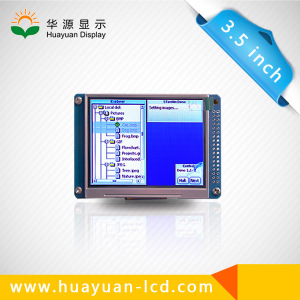
\includegraphics[width=400px, scale=1]{figuras/imagem_interface}
  \caption{TFT052A. Baseado em: \cite{tela_resistiva}}
\label{fig:imagem_interface}
\end{figure}

\begin{table}[ht]
\caption{TFT052A. Baseado em: \cite{tela_resistiva}}
\centering
\begin{tabular}{| l |  p{10cm} |}
\hline
Característica & Valores \\
\hline
Módulo Gráfico de LCD & Row / Orientado a Coluna Tipo de Controle \\
\hline
Módulo de unidade LCD & Multiplex \\
\hline
Marca & Huayuan \\
\hline
Luminosidade & 6 diodos emissores de luz em série \\
\hline
Definição & 320xRGBx240 (WQVGA) \\
\hline
Dimensão & 76,9x63,9x4,3 mm \\
\hline
Temperatura de funcionamento & -20ºC a 70º\\
\hline
Sistema de interface & 24 bits RGB \\
\hline
\end{tabular}
\label{table:table_tela_resistiva}
\end{table}

\item \textbf{TFT 054A}
O modelo TFT 054A é uma tela que pode ser usada para vigilância, celular,
carros e outras aplicações, tem display Táctil e tempo de resposra de 4 ms,
seu preço varia de 7,00 a 9,00 dolares \cite{tft}. A tabela \ref{table:table_tela_resistiva} e a figura
\ref{fig:imagem_interface2}, ilustram
as características dessa tela.

\begin{figure}[h]
  \centering
  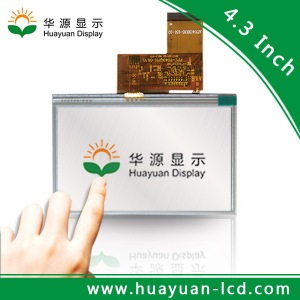
\includegraphics[width=400px, scale=1]{figuras/imagem_interface2}
  \caption{Especificações do TFT 054A. Baseado em: \cite{tft}}
\label{fig:imagem_interface2}
\end{figure}

\begin{table}[ht]
\caption{Especificações do TFT 054A. Baseado em: \cite{tft}}
\centering
\begin{tabular}{| l |  p{10cm} |}
\hline
Característica & Valores \\
\hline
Marca & Huayuan \\
\hline
Arranjo de pixel & RGB faixa vertical \\
\hline
Dimensões & 105,5x67,2x2,9 mm \\
\hline
Luz de fundo & LED branco \\
\hline
Interface do sistema & 24 bit RGB \\
\hline
Garantia & 12 meses \\
\hline
Consumo & 79,2mW \\
\hline
\end{tabular}
\label{table:table_tela_resistiva}
\end{table}


\item \textbf{FT 087A}
O modelo TFT 087A é de uso LCM de tamanho pequeno, é uma tela resisitiva
e tem tempo de resposta de 3 ms. Seu preço varia de 7,00 a 9,00 dólares
\cite{monitor_lcd}.  Na tabela \ref{table:table_tft87a}, estão as especificações
do produto e a figura \ref{fig:tft87a} é a imagem do mesmo.


\begin{figure}[h]
  \centering
  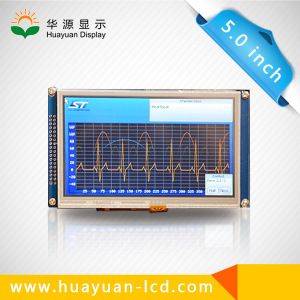
\includegraphics[width=400px, scale=1]{figuras/tela_87a}
  \caption{TFT 087A \cite{monitor_lcd}}
\label{fig:tela_87a}
\end{figure}

\begin{table}[ht]
\caption{Especificações do TFT 087A. Baseado em: \cite{monitor_lcd}}
\centering
\begin{tabular}{| l |  p{10cm} |}
\hline
Característica & Valores \\
\hline
Marca & Huayuan \\
\hline
Tipo do LCD & Branco normal transmissivo de TFT \\
\hline
Arranjos de pixel & Listra vertical do RGB \\
\hline
Dimensões & 120,7x75,8x3,1 mm \\
\hline
Garantia & 12 meses \\
\hline
\end{tabular}
\label{table:table_tft87a}
\end{table}

\item \textbf{Conclusão}
Por meio das pesquisas, foi constatado que as telas têm valores de restrição
 muito parecidos, além de estarem na mesma faixa de preço. Dessa forma, a
  tela escolhida foi a TFT054A, porque, além de ter um menor preço em relação a
  TFT052A, tem mais aplicabilidades em relação as duas outras telas citadas.
\end{enumerate}
